\documentclass[10pt]{article}
\usepackage[utf8]{inputenc}
\usepackage[portuguese]{babel}

\title{IF755 - Realidade Virtual}
\author{Vinícius Scala}
\date{April 2019}

\usepackage{natbib}
\usepackage{graphicx}

\begin{document}

\maketitle

\section{Introdução}
Realidade virtual é uma cadeira eletiva com 75 horas de carga horária e está dentro da área de mídias e interfaces.
O conceito básico de realidade virtual é a imersão sensorial em um ambiente gerado por computador. Isso pode incluir a visão, audição, tato e até olfato. Este é basicamente um tipo de simulação de realidade controlável.\cite{intro}


\begin{figure}[h!]
\centering
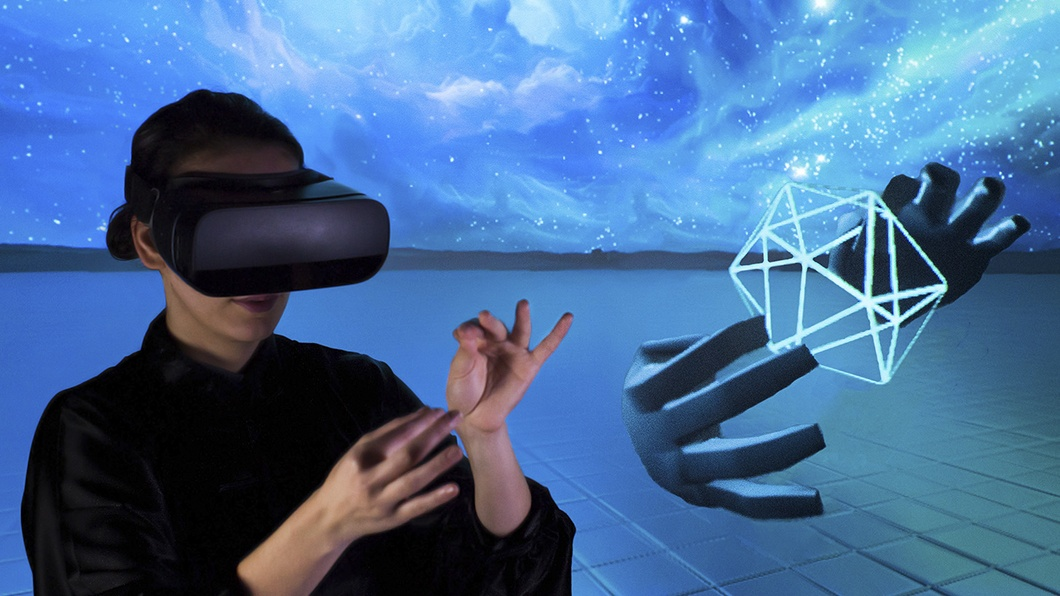
\includegraphics[scale=0.3]{vsob.jpg}
\caption{Exemplo de realidade aumentada}\cite{imagem}
\label{fig:vsob}
\end{figure}

\section{Relevância}
Realidade virtual é usada tanto como uma ferramenta como também para fins de entretenimento. A tecnologia tem muitas aplicações, como por exemplo:\\\\
Arquitetura Virtual \\
Visualização arquitetônica é um dos usos aplicados de realidade virtual hoje. Um passeio através virtual de um projeto de construção , antes de sua construção, pode realmente ajudar a arquitetos e seus clientes a entender melhor o que o edifício vai ser realmente como a habitar uma vez construído.\cite{importancia} \\\\
Treinamento de Pilotos \\
a formação de pilotos para a indústria aeronáutica é outro uso popular de realidade virtual hoje. Isso é especialmente benéfico para pilotos de avião voando aviões comerciais simuladas , pois oferece a possibilidade de praticar algo que é relativamente arriscado e caro com um avião real . Condutores de trem no Japão também treinar com simuladores de realidade virtual . \cite{importancia}


\section{Relação}

\begin{center}
\begin{tabular}{|c|p{7cm}|}
\hline
códigos & relações \\ \hline
 IF681 - Interfaces usuário-maquina &
 Nesta disciplina são demonstrados conceitos ainda básicos de design de interação e design thinking para a concepção de sistemas computacionais interativos.\cite{IF681}
 \\ \hline
  IF687 - Introdução à Multimídia  & 
Basicamente e o primeiro contato com o mundo virtual e de aplicações de multimídia vem desta disciplina seus objetivos são desenvolver a capacidade de propor e criar e avaliar mundos virtuais ênfase na internet, visando aplicações em medicina por exemplo
Desenvolver também a capacidade de especificar, construir e avaliar componentes multimídia específicos para esses mundos. \cite{IF687}
\\ \hline

\end{tabular}    
\end{center}

\bibliographystyle{plain}
\bibliography{vsob}
\end{document}
